\section{Modello Concettuale}\label{sec:modello-concettuale}
\begin{figure}[ht]
\centering
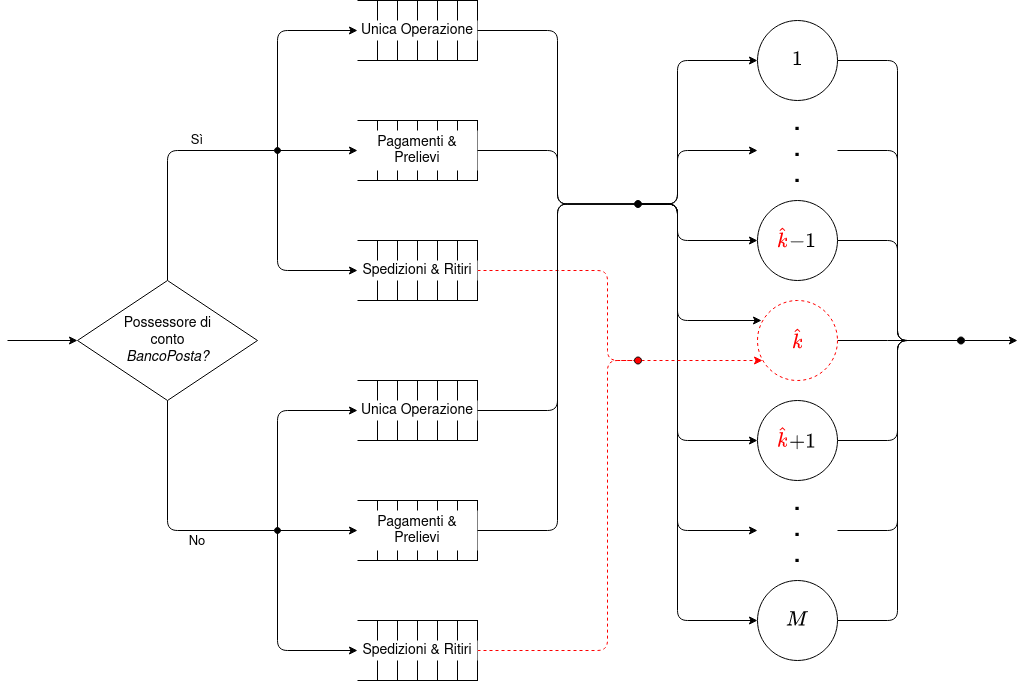
\includegraphics[width=\linewidth]{modello-concettuale-1}
\scaption{Diagramma del sistema \textbf{Poste Italiane}}
\label{fig:modello-concettuale-1}
\end{figure}

Il funzionamento del sistema è illustrato dal diagramma in figura \ref{fig:modello-concettuale-1}. Di seguito è riportata una descrizione degli elementi in esso utilizzati:
\begin{itemize}
\item Il rombo rappresenta un meccanismo di ripartizione del flusso in ingresso nelle opportune code, a seconda della titolarità o meno di un conto \textsl{BancoPosta} da parte dei clienti.
\item Ciascuna coda modella una fila di clienti possessori dello stesso tipo di ticket.
\item Ciascun servente rappresenta uno sportello dell'ufficio postale
\begin{itemize}
\item Il $k$-esimo servente (evidenziato in {\color{red} rosso}) rappresenta lo sportello dedicato per la gestione dei ticket di tipo \sr{}, il cui comportamento è stato già illustrato nel flow chart in figura \ref{fig:presentazione-1}.
\end{itemize}
\end{itemize}

Ad ogni istante di tempo, lo stato del sistema è univocamente determinato dai valori assunti dalle seguenti variabili di stato:
\begin{itemize}
\item Per ciascun servente $i$ (con $i \in \lbrace 1, 2, \dots, k-1, k+1, \dots, M \rbrace$) si ha:
\begin{equation}
Sportello_i \in \lbrace \mathtt{IDLE},\ \mathtt{BUSY} \rbrace 
\end{equation}
\item Per il $k$-esimo servente, ovvero quello dedicato, si ha:
\begin{equation}
Sportello_k \in \lbrace \mathtt{IDLE},\ \mathtt{BUSY\_GENERAL},\ \mathtt{BUSY\_SPED\_RIT}\rbrace 
\end{equation}
dove:
\begin{itemize}
\item \texttt{BUSY\_GENERAL} rappresenta il caso in cui il servente stia elaborando un ticket \textbf{non} di tipo \sr{}.
\item \texttt{BUSY\_SPED\_RIT} rappresenta il caso in cui il servente stia elaborando un ticket di tipo \sr{}.
\end{itemize}
\item Per ciascuna coda $(t, j)$ con:
\begin{itemize}
\item $t \in \lbrace \mathtt{BANCO\_POSTA},\ \mathtt{STANDARD}\rbrace$
\item $j \in \lbrace \mathtt{UNICA\_OP},\ \mathtt{PAGAM\_PREL},\ \mathtt{SPED\_RIT} \rbrace$
\end{itemize}
il numero di clienti in essa presenti è modellato da $Coda_{t,j} \in \mathbb{N}$.
\end{itemize}
